\chapter{Material}
\label{ch:Material}
\enlargethispage{120cm}
\section{Pmod-Pinbelegung für die Event-Aufnahme}
\label{sec:pmod_pins}
Für die Event-Aufnahme sind die Pmod-Header P3 und P4 als Eingänge konfiguriert.

\begin{figure}[h]
	\centering
	\captionsetup{justification=centering,margin=2cm}
		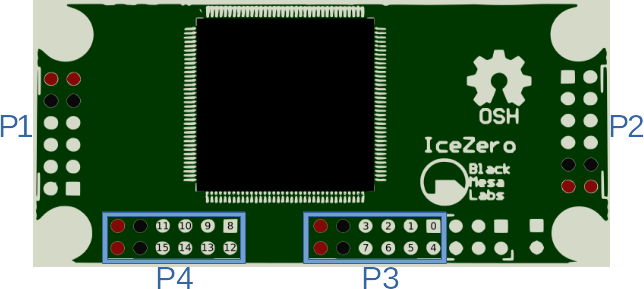
\includegraphics[width=0.80\textwidth]{../figures/ice40_pmod_pins_01.png}
		\caption[Pinbelegung der Pmod-Header des IceZero-Boards]{Pinbelegung der Pmod-Header des IceZero-Boards}
	\label{fig:ice40_pmod_pins}
\end{figure}

Bei der Pin-Belegung wurde das selbe Schema wie beim GPIO-Modul des IcoSoc verwendet. Die Numerierung läuft dementsprechend von rechts nach links und für die einzelnen Pmod-Header ``zeilenweise'' von oben nach unten.\\
Für die Zuordnung der Signalnamen (und der zugehörigen VCD-Symbole) bei der Ausgabe im CSV- oder VCD-Format kann folgende Tabelle verwendet werden:

\begin{table}[h]
\centering
\resizebox{\columnwidth}{!}{%

\begin{tabular}{lllllllclllll}
\cline{3-6} \cline{10-13}
                                                   & \multicolumn{1}{l|}{}                                                   & \multicolumn{1}{c|}{\cellcolor[HTML]{EFEFEF},}       & \multicolumn{1}{c|}{\cellcolor[HTML]{EFEFEF}+}       & \multicolumn{1}{c|}{\cellcolor[HTML]{EFEFEF}*}       & \multicolumn{1}{c|}{\cellcolor[HTML]{EFEFEF})}       & \multicolumn{1}{c}{}  &                                                   & \multicolumn{1}{c|}{}                                                   & \multicolumn{1}{c|}{\cellcolor[HTML]{EFEFEF}\$}     & \multicolumn{1}{c|}{\cellcolor[HTML]{EFEFEF}\#}     & \multicolumn{1}{c|}{\cellcolor[HTML]{EFEFEF}"}      & \multicolumn{1}{c|}{\cellcolor[HTML]{EFEFEF}!}      \\ \cline{1-6} \cline{8-13} 
\multicolumn{1}{|l|}{\cellcolor[HTML]{DF2727}3.3V} & \multicolumn{1}{l|}{\cellcolor[HTML]{343434}{\color[HTML]{FFFFFF} GND}} & \multicolumn{1}{l|}{\cellcolor[HTML]{C0C0C0}pin\_11} & \multicolumn{1}{l|}{\cellcolor[HTML]{C0C0C0}pin\_10} & \multicolumn{1}{l|}{\cellcolor[HTML]{C0C0C0}pin\_9}  & \multicolumn{1}{l|}{\cellcolor[HTML]{C0C0C0}pin\_8}  & \multicolumn{1}{l|}{} & \multicolumn{1}{l|}{\cellcolor[HTML]{DF2727}3.3V} & \multicolumn{1}{l|}{\cellcolor[HTML]{343434}{\color[HTML]{FFFFFF} GND}} & \multicolumn{1}{l|}{\cellcolor[HTML]{C0C0C0}pin\_3} & \multicolumn{1}{l|}{\cellcolor[HTML]{C0C0C0}pin\_2} & \multicolumn{1}{l|}{\cellcolor[HTML]{C0C0C0}pin\_1} & \multicolumn{1}{l|}{\cellcolor[HTML]{C0C0C0}pin\_0} \\ \cline{1-6} \cline{8-13} 
\multicolumn{1}{|l|}{\cellcolor[HTML]{DF2727}3.3V} & \multicolumn{1}{l|}{\cellcolor[HTML]{343434}{\color[HTML]{FFFFFF} GND}} & \multicolumn{1}{l|}{\cellcolor[HTML]{C0C0C0}pin\_15} & \multicolumn{1}{l|}{\cellcolor[HTML]{C0C0C0}pin\_14} & \multicolumn{1}{l|}{\cellcolor[HTML]{C0C0C0}pin\_13} & \multicolumn{1}{l|}{\cellcolor[HTML]{C0C0C0}pin\_12} & \multicolumn{1}{l|}{} & \multicolumn{1}{l|}{\cellcolor[HTML]{DF2727}3.3V} & \multicolumn{1}{l|}{\cellcolor[HTML]{343434}{\color[HTML]{FFFFFF} GND}} & \multicolumn{1}{l|}{\cellcolor[HTML]{C0C0C0}pin\_7} & \multicolumn{1}{l|}{\cellcolor[HTML]{C0C0C0}pin\_6} & \multicolumn{1}{l|}{\cellcolor[HTML]{C0C0C0}pin\_5} & \multicolumn{1}{l|}{\cellcolor[HTML]{C0C0C0}pin\_4} \\ \cline{1-6} \cline{8-13} 
                                                   & \multicolumn{1}{l|}{}                                                   & \multicolumn{1}{c|}{\cellcolor[HTML]{EFEFEF}0}       & \multicolumn{1}{c|}{\cellcolor[HTML]{EFEFEF}/}       & \multicolumn{1}{c|}{\cellcolor[HTML]{EFEFEF}.}       & \multicolumn{1}{c|}{\cellcolor[HTML]{EFEFEF}-}       & \multicolumn{1}{c}{}  &                                                   & \multicolumn{1}{c|}{}                                                   & \multicolumn{1}{c|}{\cellcolor[HTML]{EFEFEF}(}      & \multicolumn{1}{c|}{\cellcolor[HTML]{EFEFEF}'}      & \multicolumn{1}{c|}{\cellcolor[HTML]{EFEFEF}\&}     & \multicolumn{1}{c|}{\cellcolor[HTML]{EFEFEF}\%}     \\ \cline{3-6} \cline{10-13} 
\multicolumn{6}{c}{Pmod - P4}                                                                                                                                                                                                                                                                                                                            &                       & \multicolumn{6}{c}{Pmod - P3}                                                                                                                                                                                                                                                                                                                      
\end{tabular}

%\begin{tabular}{lllllllllllll}
%\cline{1-6} \cline{8-13}
%\multicolumn{1}{|l|}{\cellcolor[HTML]{DF2727}3.3V} & \multicolumn{1}{l|}{\cellcolor[HTML]{343434}{\color[HTML]{FFFFFF} GND}} & \multicolumn{1}{l|}{pin\_11} & \multicolumn{1}{l|}{pin\_10} & \multicolumn{1}{l|}{pin\_9}  & \multicolumn{1}{l|}{pin\_8}  & \multicolumn{1}{l|}{} & \multicolumn{1}{l|}{\cellcolor[HTML]{DF2727}3.3V} & \multicolumn{1}{l|}{\cellcolor[HTML]{343434}{\color[HTML]{FFFFFF} GND}} & \multicolumn{1}{l|}{pin\_3} & \multicolumn{1}{l|}{pin\_2} & \multicolumn{1}{l|}{pin\_1} & \multicolumn{1}{l|}{pin\_0} \\ \cline{1-6} \cline{8-13} 
%\multicolumn{1}{|l|}{\cellcolor[HTML]{DF2727}3.3V} & \multicolumn{1}{l|}{\cellcolor[HTML]{343434}{\color[HTML]{FFFFFF} GND}} & \multicolumn{1}{l|}{pin\_15} & \multicolumn{1}{l|}{pin\_14} & \multicolumn{1}{l|}{pin\_13} & \multicolumn{1}{l|}{pin\_12} & \multicolumn{1}{l|}{} & \multicolumn{1}{l|}{\cellcolor[HTML]{DF2727}3.3V} & \multicolumn{1}{l|}{\cellcolor[HTML]{343434}{\color[HTML]{FFFFFF} GND}} & \multicolumn{1}{l|}{pin\_7} & \multicolumn{1}{l|}{pin\_6} & \multicolumn{1}{l|}{pin\_5} & \multicolumn{1}{l|}{pin\_4} \\ \cline{1-6} \cline{8-13} 
%\multicolumn{6}{c}{Pmod - P4}                                                                                                                                                                                                                            &                       & \multicolumn{6}{c}{Pmod - P3}                                                                                                                                                                                                                      
%\end{tabular}
}
\caption{Pinbelegung der Pmod-Header des Icezero-Boards}
\label{tbl:Pmod-Pins}
\end{table}


\clearpage
\begin{landscape}

\section{Pinverbindungen Raspberry Pi und IceZero FPGA-Shield}

Bei den mit einem ``X'' markierten Pins besteht Hardware-seitig keine Verbindung zwischen dem Raspberry Pi und dem IceZero-Board.

\begin{table}[h]
\centering
%\resizebox{\textwidth}{!}{%
\begin{tabular}{|c|c|c|c|c|
>{\columncolor[HTML]{EFEFEF}}c |
>{\columncolor[HTML]{EFEFEF}}c |c|c|c|c|c|}
\hline
\cellcolor[HTML]{C0C0C0}Funktion & \cellcolor[HTML]{C0C0C0}iCE40 & \cellcolor[HTML]{C0C0C0}IceZero & \cellcolor[HTML]{C0C0C0}WiringPi & \cellcolor[HTML]{C0C0C0}Name                        & \multicolumn{2}{c|}{\cellcolor[HTML]{C0C0C0}Physical} & \cellcolor[HTML]{C0C0C0}Name                       & \cellcolor[HTML]{C0C0C0}WiringPi & \cellcolor[HTML]{C0C0C0}IceZero & \cellcolor[HTML]{C0C0C0}iCE40 & \cellcolor[HTML]{C0C0C0}Funktion \\ \hline
                                 &                               &                                 &                                  & \cellcolor[HTML]{DF2727}3.3V                        & 1                         & 2                         & \cellcolor[HTML]{DF2727}5V                         &                                  &                                 &                               &                                  \\ \hline
unused                           & 115                           & PI\_I2C\_SDA                    & 8                                & SDA.1                                               & 3                         & 4                         & \cellcolor[HTML]{DF2727}5V                         &                                  &                                 &                               &                                  \\ \hline
unused                           & 114                           & PI\_I2C\_SCL                    & 9                                & SCL.1                                               & 5                         & 6                         & \cellcolor[HTML]{333333}{\color[HTML]{FFFFFF} GND} &                                  &                                 &                               &                                  \\ \hline
                                 &                               & {\color[HTML]{000000} X}        & 7                                & 1-Wire                                              & 7                         & 8                         & TxD                                                & 15                               & PI\_UART\_WI                    & 113                           & DEBUG\_UART                      \\ \hline
                                 &                               &                                 &                                  & \cellcolor[HTML]{333333}{\color[HTML]{FFFFFF} GND}  & 9                         & 10                        & RxD                                                & 16                               & PI\_UART\_RO                    & 112                           & DEBUG\_UART                      \\ \hline
                                 &                               & X                               & 0                                & GPIO.0                                              & 11                        & 12                        & GPIO.1                                             & 1                                & X                               &                               &                                  \\ \hline
                                 &                               & X                               & 2                                & GPIO.2                                              & 13                        & 14                        & \cellcolor[HTML]{333333}{\color[HTML]{FFFFFF} GND} &                                  &                                 &                               &                                  \\ \hline
unused                           & 101                           & PI\_GPIO\_2                     & 3                                & GPIO.3                                              & 15                        & 16                        & GPIO.4                                             & 4                                & X                               &                               &                                  \\ \hline
                                 &                               &                                 &                                  & \cellcolor[HTML]{DF2727}{\color[HTML]{000000} 3.3V} & 17                        & 18                        & GPIO.5                                             & 5                                & PI\_GPIO\_1                     & 99                            & unused                           \\ \hline
DATA\_MOSI                       & 90                            & PI\_SPI\_MOSI                   & 12                               & MOSI                                                & 19                        & 20                        & \cellcolor[HTML]{333333}{\color[HTML]{FFFFFF} GND} &                                  &                                 &                               &                                  \\ \hline
DATA\_MISO                       & 87                            & PI\_SPI\_MISO                   & 13                               & MISO                                                & 21                        & 22                        & GPIO.6                                             & 6                                & PI\_GPIO\_0                     & 88                            & unused                           \\ \hline
DATA\_SCK                        & 79                            & PI\_SPI\_SCK                    & 14                               & SCLK                                                & 23                        & 24                        & CE0                                                & 10                               & PI\_SPI\_CE\_0                  & 85                            & DATA\_SS                         \\ \hline
                                 &                               &                                 &                                  & \cellcolor[HTML]{333333}{\color[HTML]{FFFFFF} GND}  & 25                        & 26                        & CE1                                                & 11                               & PI\_SPI\_CE\_1                  & 78                            & unused                           \\ \hline
unused                           & 73                            & PI\_ID\_0                       & 30                               & SDA.0                                               & 27                        & 28                        & SCL.0                                              & 31                               & PI\_ID\_1                       & 74                            & unused                           \\ \hline
CONFIG\_DONE                     & 65                            & CFG\_DONE                       & 21                               & GPIO.21                                             & 29                        & 30                        & \cellcolor[HTML]{333333}{\color[HTML]{FFFFFF} GND} &                                  &                                 &                               &                                  \\ \hline
CONFIG\_MOSI                     & 68                            & CFG\_SI                         & 22                               & GPIO.22                                             & 31                        & 32                        & GPIO.26                                            & 26                               & CFG\_SS                         & 71                            & CONFIG\_SS                       \\ \hline
CONFIG\_MISO                     & 67                            & CFG\_SO                         & 23                               & GPIO.23                                             & 33                        & 34                        & \cellcolor[HTML]{333333}{\color[HTML]{FFFFFF} GND} &                                  &                                 &                               &                                  \\ \hline
                                 &                               & X                               & 24                               & GPIO.24                                             & 35                        & 36                        & GPIO.27                                            & 27                               & CFG\_SCK                        & 70                            & CONFIG\_SCK                      \\ \hline
CONFIG\_RESET                    & 66                            & CFG\_RST\_1                     & 25                               & GPIO.25                                             & 37                        & 38                        & GPIO.28                                            & 28                               & X                               &                               &                                  \\ \hline
                                 &                               &                                 &                                  & \cellcolor[HTML]{333333}{\color[HTML]{FFFFFF} GND}  & 39                        & 40                        & GPIO.29                                            & 29                               & X                               &                               &                                  \\ \hline
\end{tabular}%
%}
\caption{Pinverbindungen Raspberry Pi und IceZero FPGA-Shield}
\label{tbl:pins}
\end{table}
\end{landscape}

\clearpage
\section{Detaillierte Pinbelegung aller Pmod-Header}
\label{sec:pmod_all}

%Pmod1
\begin{table}[H]
\centering
\caption{Pinbelegung Pmod-P1}
\label{tbl:pmod1}
\begin{tabular}{|l|l|l|l|l|}
\hline
\cellcolor[HTML]{EFEFEF}130       & \cellcolor[HTML]{EFEFEF}135      & \cellcolor[HTML]{EFEFEF}137      & \cellcolor[HTML]{EFEFEF}139      & iCE40 PCF Pin \\ \hline
GPIO\_PIN\_7                      & GPIO\_PIN\_5                     & GPIO\_PIN\_3                     & GPIO\_PIN\_1                     & IceZero Name  \\ \hline
\cellcolor[HTML]{C0C0C0}pmod1\_4  & \cellcolor[HTML]{C0C0C0}pmod1\_3 & \cellcolor[HTML]{C0C0C0}pmod1\_2 & \cellcolor[HTML]{C0C0C0}pmod1\_1 & IcoSoc Name   \\ \hline
\cellcolor[HTML]{C0C0C0}pmod1\_10 & \cellcolor[HTML]{C0C0C0}pmod1\_9 & \cellcolor[HTML]{C0C0C0}pmod1\_8 & \cellcolor[HTML]{C0C0C0}pmod1\_7 & IcoSoc Name   \\ \hline
GPIO\_PIN\_6                      & GPIO\_PIN\_4                     & GPIO\_PIN\_2                     & GPIO\_PIN\_0                     & IceZero Name  \\ \hline
\cellcolor[HTML]{EFEFEF}134       & \cellcolor[HTML]{EFEFEF}136      & \cellcolor[HTML]{EFEFEF}138      & \cellcolor[HTML]{EFEFEF}141      & iCE40 PCF Pin \\ \hline
\multicolumn{5}{|c|}{Pmod P1}                                                                                                                              \\ \hline
\end{tabular}
\end{table}

%Pmod2
\begin{table}[H]
\centering
\caption{Pinbelegung Pmod-P2}
\label{tbl:pmod2}
\begin{tabular}{|l|l|l|l|l|}
\hline
\cellcolor[HTML]{EFEFEF}43        & \cellcolor[HTML]{EFEFEF}45       & \cellcolor[HTML]{EFEFEF}48       & \cellcolor[HTML]{EFEFEF}56       & iCE40 PCF Pin \\ \hline
GPIO\_PIN\_15                     & GPIO\_PIN\_13                    & GPIO\_PIN\_11                    & GPIO\_PIN\_9                     & IceZero Name  \\ \hline
\cellcolor[HTML]{C0C0C0}pmod2\_4  & \cellcolor[HTML]{C0C0C0}pmod2\_3 & \cellcolor[HTML]{C0C0C0}pmod2\_2 & \cellcolor[HTML]{C0C0C0}pmod2\_1 & IcoSoc Name   \\ \hline
\cellcolor[HTML]{C0C0C0}pmod2\_10 & \cellcolor[HTML]{C0C0C0}pmod2\_9 & \cellcolor[HTML]{C0C0C0}pmod2\_8 & \cellcolor[HTML]{C0C0C0}pmod2\_7 & IcoSoc Name   \\ \hline
GPIO\_PIN\_14                     & GPIO\_PIN\_12                    & GPIO\_PIN\_10                    & GPIO\_PIN\_8                     & IceZero Name  \\ \hline
\cellcolor[HTML]{EFEFEF}42        & \cellcolor[HTML]{EFEFEF}44       & \cellcolor[HTML]{EFEFEF}47       & \cellcolor[HTML]{EFEFEF}55       & iCE40 PCF Pin \\ \hline
\multicolumn{5}{|c|}{Pmod P2}                                                                                                                              \\ \hline
\end{tabular}
\end{table}

%Pmod3

\begin{table}[H]
\centering
\caption{Pinbelegung Pmod-P3}
\label{tbl:pmod3}
\begin{tabular}{|l|l|l|l|l|}
\hline
\cellcolor[HTML]{EFEFEF}52        & \cellcolor[HTML]{EFEFEF}28       & \cellcolor[HTML]{EFEFEF}29       & \cellcolor[HTML]{EFEFEF}26       & iCE40 PCF Pin \\ \hline
GPIO\_PIN\_31                     & GPIO\_PIN\_30                    & GPIO\_PIN\_29                    & GPIO\_PIN\_28                    & IceZero Name  \\ \hline
\cellcolor[HTML]{C0C0C0}pmod3\_4  & \cellcolor[HTML]{C0C0C0}pmod3\_3 & \cellcolor[HTML]{C0C0C0}pmod3\_2 & \cellcolor[HTML]{C0C0C0}pmod3\_1 & IcoSoc Name   \\ \hline
\cellcolor[HTML]{C0C0C0}pmod3\_10 & \cellcolor[HTML]{C0C0C0}pmod3\_9 & \cellcolor[HTML]{C0C0C0}pmod3\_8 & \cellcolor[HTML]{C0C0C0}pmod3\_7 & IcoSoc Name   \\ \hline
GPIO\_PIN\_19                     & GPIO\_PIN\_18                    & GPIO\_PIN\_17                    & GPIO\_PIN\_16                    & IceZero Name  \\ \hline
\cellcolor[HTML]{EFEFEF}37        & \cellcolor[HTML]{EFEFEF}38       & \cellcolor[HTML]{EFEFEF}39       & \cellcolor[HTML]{EFEFEF}41       & iCE40 PCF Pin \\ \hline
\multicolumn{5}{|c|}{Pmod P3}                                                                                                                              \\ \hline
\end{tabular}
\end{table}

%Pmod4

\begin{table}[H]
\centering
\caption{Pinbelegung Pmod-P4}
\label{tbl:pmod4}
\begin{tabular}{|l|l|l|l|l|}
\hline
\cellcolor[HTML]{EFEFEF}7         & \cellcolor[HTML]{EFEFEF}8        & \cellcolor[HTML]{EFEFEF}20       & \cellcolor[HTML]{EFEFEF}21       & iCE40 PCF Pin      \\ \hline
GPIO\_PIN\_27                     & GPIO\_PIN\_26                    & GPIO\_PIN\_25                    & GPIO\_PIN\_24                    & IceZero Name \\ \hline
\cellcolor[HTML]{C0C0C0}pmod4\_4  & \cellcolor[HTML]{C0C0C0}pmod4\_3 & \cellcolor[HTML]{C0C0C0}pmod4\_2 & \cellcolor[HTML]{C0C0C0}pmod4\_1 & IcoSoc Name  \\ \hline
\cellcolor[HTML]{C0C0C0}pmod4\_10 & \cellcolor[HTML]{C0C0C0}pmod4\_9 & \cellcolor[HTML]{C0C0C0}pmod4\_8 & \cellcolor[HTML]{C0C0C0}pmod4\_7 & IcoSoc Name  \\ \hline
GPIO\_PIN\_23                     & GPIO\_PIN\_22                    & GPIO\_PIN\_21                    & GPIO\_PIN\_20                    & IceZero Name \\ \hline
\cellcolor[HTML]{EFEFEF}142       & \cellcolor[HTML]{EFEFEF}143      & \cellcolor[HTML]{EFEFEF}144      & \cellcolor[HTML]{EFEFEF}1        & iCE40 PCF Pin      \\ \hline
\multicolumn{5}{|c|}{Pmod P4}                                                                                                                             \\ \hline
\end{tabular}
\end{table}

\clearpage

\section{Inhalt der CD}
Die beiliegende CD enthält den Inhalt des Github-Repositories 
\begin{lstlisting}[language=bash]
https://github.com/dm7h/fpga-event-recorder
\end{lstlisting}
zum Zeitpunkt der Abgabe.

Die folgende Tabelle bietet einen Überblick über die Inhalte des Repositories:
\begin{table}[h]
\centering

\begin{tabular}{|p{1cm}|p{3cm}|p{10cm}|}
\hline
\rowcolor[HTML]{C0C0C0} 
Verz. & Unterverzeichnis                & Inhaltsbeschreibung                                                                                                                                                                                                                                                                                                      \\ \hline
thesis/     &                                 & Finale Version der Bachelorarbeit als PDF                                                                                                                                                                                                                                                             \\ \hline
thesis/     & src/                            & Latex-Sourcen der Bachelorarbeit                                                                                                                                                                                                                                                              \\ \hline
doc/        & ref/                            & iCE40 Manuals und relevante Hardwaredokumentation                                                                                                                                                                                                                                                                        \\ \hline
misc/       &                                 & Nicht direkt Event-Recorder bezogene Informationen und  Code (u.a. für die Analyse)                                                                                                                                                                                                                                                             \\ \hline
src/        &                                 &                                                                                                                                                                                                                                                                                                                          \\ \hline
            & Logikanalysator/                & Dateien des Semesterprojekts ``Logikanalysator mit AVR Mega32U4 und Altera MAX CPLD''  inkl. Dateien der Bachelorarbeit von Andreas Müller (USB-TPLE)  
															     \\ \hline
            & icotools/                       & Portierung des icotools Projekts für das IceZero-Board. Original-Repository: https://github.com/cliffordwolf/icotools. Relevant sind hier vor allem die Unterverzeichnisse ``icosoc'' und ``icozprog'' 
\\ \hline
            & icozctl/                        & Fork des icoprog-Tools (icotools/icoporg) mit zusätzlichen Funktionen zur Steuerung des Event-Recorders                                                                                                                                                                                                                  \\ \hline
            & picosoc/                        & Portierung des PicoSoc-Projekts auf das IceZero-Board (nicht direkt projekt-relevant). PicoSoc ist eine minimale Variante des IcoSocs. Original-Repository: https://github.com/cliffordwolf/picorv32/tree/master/picosoc                                                    \\ \hline
            & sump2\_ice40/                          & SUMP2 Variante für das IceZero-Board. Quelle: https://blackmesalabs.wordpress.com/2017/02/07/icezero-fpga-board-for-rasppi/                                                                                                                                                                                                                                                    \\ \hline
            & sump2\_pipistrello\_ ftdi\_fifo/ & SUMP2 Vairante für das Pipistrello-Board bei dem der UART durch einen FTDI-Fifo ersetzt wurde, um einen Höheren Datenduchsatz zu ermöglichen. Quelle: http://forum.gadgetfactory.net/topic/1748-open-bench-logic-sniffer-with-64mb-capture-buffer/ \\ \hline
            & demon-core-import/              & SUMP2 Weiterenwicklung für den Open Bench Logic Sniffer. Quelle: https://github.com/jhol/demon-core-import                                                                                                                                                                     \\ \hline
\end{tabular}
\caption{Überblick über den Inhalt des Git-Repositories}
\label{tbl:git_repo}
\end{table}
